\chapter{Background}
\textbf{Notes to self:}
I need to provide a theoretical perspective from which I can produce a clearly stated conceptual framework\cite{weinberg2006weinberg}. Use principles of a \textit{Literature review} here to set the scene.

\section{Overview of this chapter}


Failure Heatmaps: Some failures occur consistently and often. Others are affected by various factors, such as the input provided to the code, the runtime environment, API responses, etc. where the failure coincides with one or more factors. See: Concomitant Variation\cite{mill1884system} and Influencing Agents\cite{mill1884system}. One of the challenges that applies to bug localisation and bug reproduction is to discover or identify whether there are these factors, and if so how to control these factors to make the failures more likely to occur on demand (and perhaps less likely to occur when the software is in use). One of the challenges may be to identify influencing agents\cite{mill1884system} i.e. agents that influence the results such as the crash rate in order to seek ways to specify or control those agents as inputs during in bug reproduction and/or testing. As a practical example, if the version of Android seems to be an influencing agent for the crash rate for a particular crash cluster, could we find ways to control (choose) the Android version to help with identifying a relationship between the incidence of the crash and the Android version. It is possible to do so, for instance by selecting a device with the desired Android version and performing tests of the app on that device. At this stage we may still know little about the \textit{cause(s)} of the failure and there could be various contributing factors, for instance the crash may occur only on a subset of devices which have the particular Android version, until we investigate further we may not be able to identify the pattern precisely. 

\section{Testing Mobile apps}
Testing can help in various aspects, including: identifying the factors, bug localisation and reproduction, and testing the effects and outcomes of any changes made to the codebase, environment, configuration, use, \textit{etc}.

Amplify potentially problematic behaviours to expose poor behaviours in Android apps\cite{yang2013testing}. Chaos Monkey style approach in VanarSena...

Possibly mention my concept of a beaufort scale for testing (and perhaps to measure runtime environments generally?)\cite{harty_beaufort_scale_2018}

Test automation for Android apps\cite{SLR_automated_testing_android_apps_2019}

\section{Semantic gaps}
\emph{"As computer scientists, this group of academics knew that developers searching for solutions to coding questions are impaired by a lexical gap between their query (task description) and the information (lines of actual code) associated with the solution that they are looking for."}\cite{popper_crokage_2019}
 or perhaps the original paper's abstract's phrasing: 
\emph{" First, the search is impaired due to a lexical gap between their query (task description) and the information associated with the solution"}\cite{Silva:2019:RCS:3339076.3339130}

Bug localisation: \textit{TBC}
\url{https://www.overleaf.com/project/5cbc30a12722015859bc5e8a}

Finding crashes in Android apps: 

\subsection{Adding diagnostic data to crashes}

\begin{figure}
    \centering
    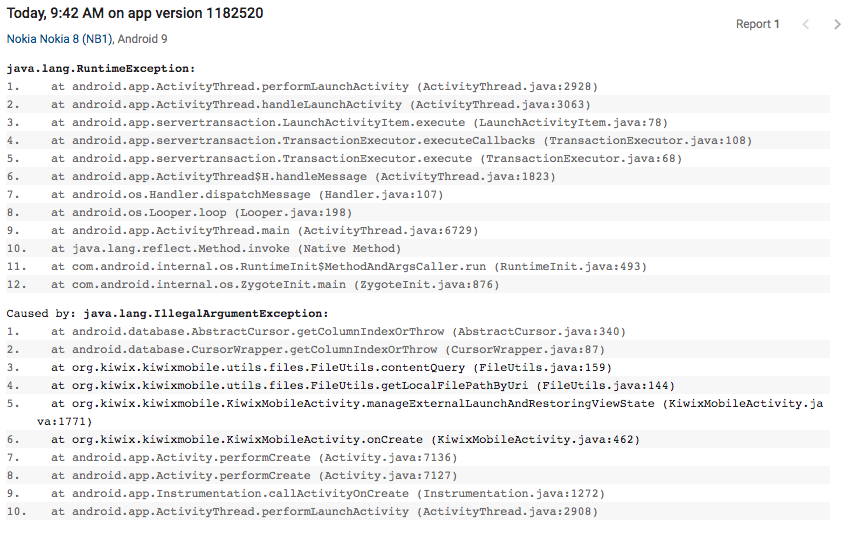
\includegraphics[angle=90,origin=c,trim={0.2cm 0 0.8cm 0},clip, width=\textwidth,height=\textheight,keepaspectratio]{images/PHeT_Example_Crash_StackTrace(2019-Jun-14).png}
    \caption{Example of a reported crash for the Chemistry \& Physics simulations app}
    \label{fig:phet_stack_trace}
\end{figure}
% I've only followed the basics of https://tex.stackexchange.com/questions/57418/crop-an-inserted-image There's more to discover and use!

Can we improve the diagnostic abilities of crash stacktraces? 

Figure \ref{fig:phet_stack_trace} provides an example of an individual crash trace reported in Android Vitals in one of the Kiwix family of Android apps. The crash originates with a Java exception \texttt{java.lang.IllegalArgumentException} thrown at line 159 of \texttt{FileUtils.java} (linenumber 3 of the extract of the stack trace, shown below). 

\definecolor{mygreen}{rgb}{0,0.6,0}
\definecolor{mygray}{rgb}{0.5,0.5,0.5}
\definecolor{mymauve}{rgb}{0.58,0,0.82}

\lstset{ 
  backgroundcolor=\color{white},   % choose the background color; you must add \usepackage{color} or \usepackage{xcolor}; should come as last argument
  basicstyle=\tiny,        % the size of the fonts that are used for the code
  breakatwhitespace=false,         % sets if automatic breaks should only happen at whitespace
  breaklines=true,                 % sets automatic line breaking
  captionpos=b,                    % sets the caption-position to bottom
  firstnumber=3,                % start line enumeration with line 3	                   % adds a frame around the code
  keepspaces=true,                 % keeps spaces in text, useful for keeping indentation of code (possibly needs columns=flexible)
  numbers=left,                    % where to put the line-numbers; possible values are (none, left, right)
  numbersep=5pt,                   % how far the line-numbers are from the code
  numberstyle=\tiny\color{mygray}, % the style that is used for the line-numbers
  stepnumber=1,                    % the step between two line-numbers. If it's 1, each line will be numbered
  columns=flexible,
  title=\lstname                   % show the filename of files included with \lstinputlisting; also try caption instead of title
}
% from https://en.wikibooks.org/wiki/LaTeX/Source_Code_Listings

\begin{lstlisting}
 at org.kiwix.kiwixmobile.utils.files.FileUtils.contentQuery (FileUtils.java:159)
 at org.kiwix.kiwixmobile.utils.files.FileUtils.getLocalFilePathByUri (FileUtils.java:144) 
 at org.kiwix.kiwixmobile.KiwixMobileActivity.manageExternalLaunchAndRestoringViewState (KiwixMobileActivity.java:1771)
 at org.kiwix.kiwixmobile.KiwixMobileActivity.onCreate (KiwixMobileActivity.java:462)
\end{lstlisting}

The stack trace report includes the device model, a Nokia Nokia 8 (NB1) running Android 9 which may be useful to help isolate or reproduce the crash. 

An extract of the relevant code in \texttt{KiwixMobileActivity.java} follows and shows the parameters being passed into \texttt{FileUtils.getLocalFilePathByUri}. From the stacktrace we do not have enough information to know what was passed into the method that triggered the exception. TBC

\lstset{ 
  basicstyle=\footnotesize,
  firstnumber=1767
  }
  
\begin{lstlisting}
  private void manageExternalLaunchAndRestoringViewState() {

    if (getIntent().getData() != null) {
      String filePath =
          FileUtils.getLocalFilePathByUri(getApplicationContext(), getIntent().getData());
\end{lstlisting}
\subsection{Effects of App Stores on development practices}

\subsection{Privacy, Tracking, and Visibility}
Analytics requires data to be collected somehow. The data may be captured within the app or outside it, for instance by the operating system. Tracking of users also requires data to be collected similarly; and some of the data collected for tracking may used for both tracking and analytics. Tracking is not necessarily 'bad' however there are ongoing concerns whether the tracking is necessary, a form of currency, and whether there are imbalances in what's collected vs. the privacy of users. 

Google provides a central location where users can see their activity across various Google products and services including Android \url{https://myactivity.google.com/myactivity}. They can filter the results, for instance Android related activity is available using \url{https://myactivity.google.com/myactivity?product=1}. Google provides controls \url{https://myaccount.google.com/activitycontrols} and allows users to delete their history \url{https://myactivity.google.com/delete-activity} albeit anonymous crash and other app data might be preserved in data and reports made available in Android Vitals. 

\begin{figure}
    \centering
    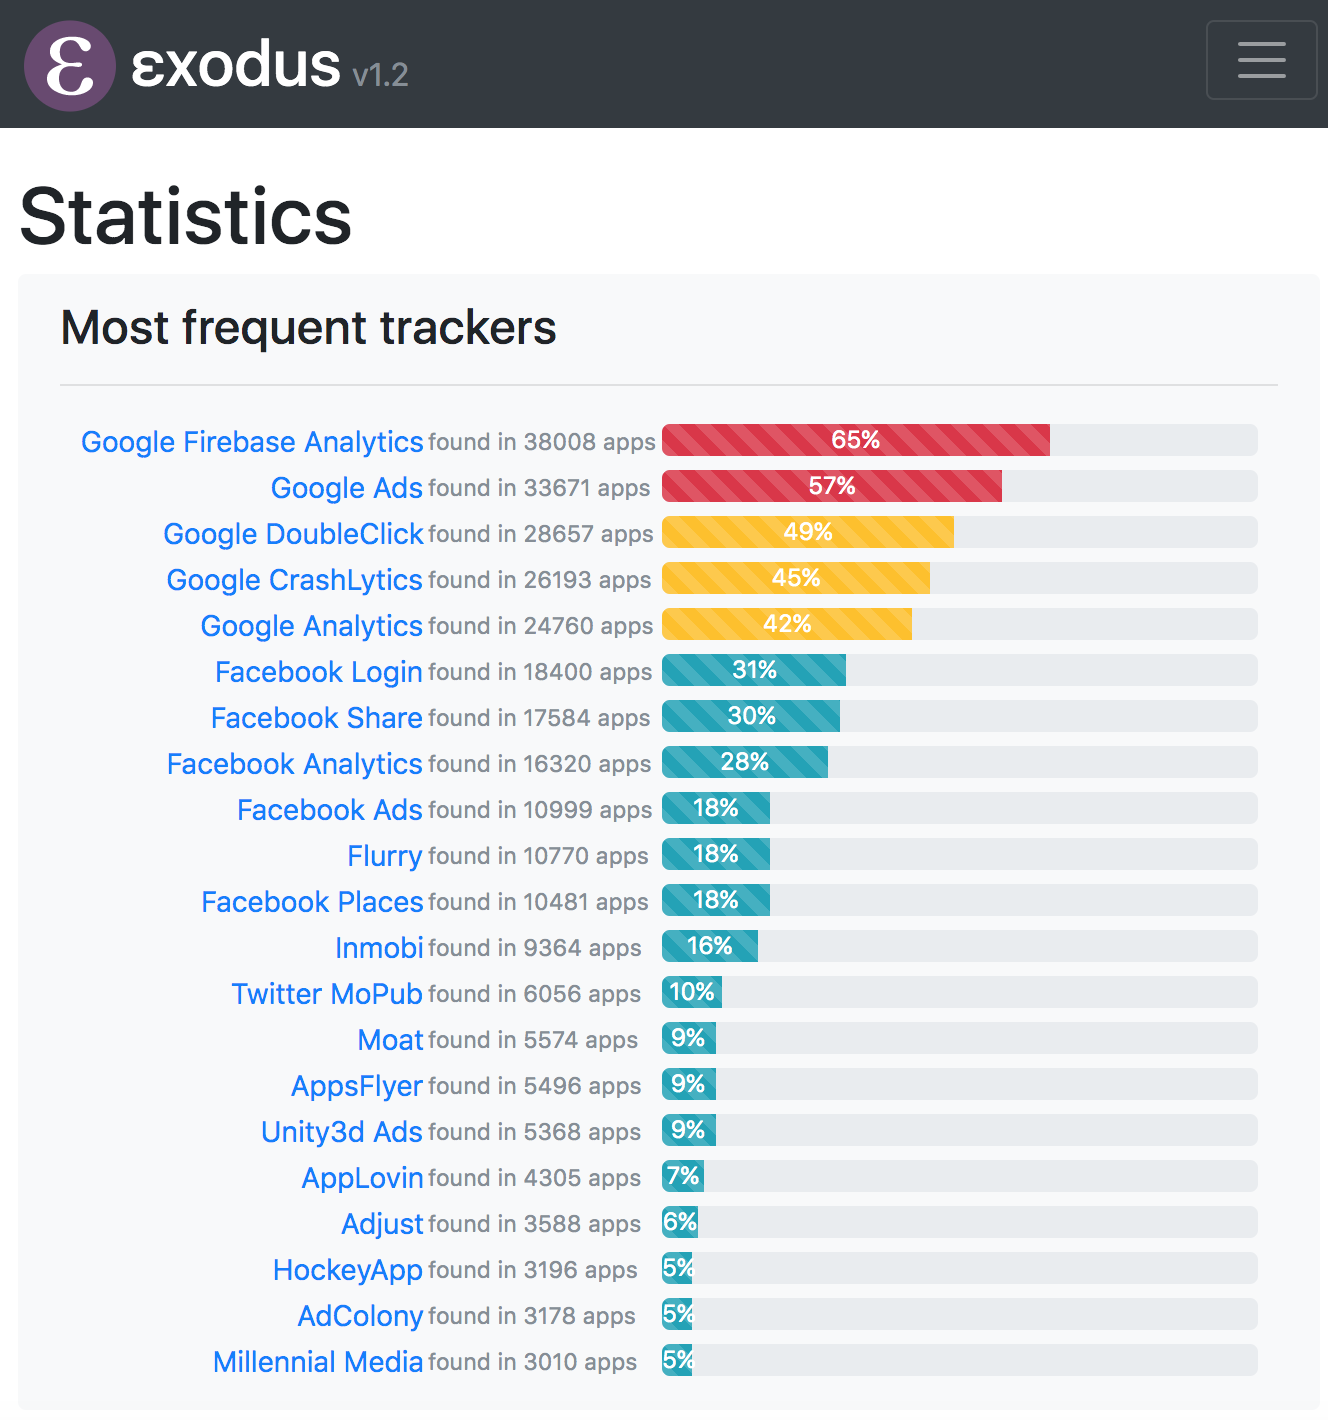
\includegraphics[width=\textwidth, height=\textheight, keepaspectratio]{images/exodus_most_frequent_trackers_14_jun_2019.png}
    \caption{Most Frequent Trackers detected by Exodus Privacy project}
    \label{fig:exodus_most_frequent_trackers}
\end{figure}

There are various streams of tracking: by the mobile operating system (Android, etc.), by Google apps (GMail, Google Assistant, Google Maps, etc.) and by other apps that use Google, Facebook, or other mobile analytics services. As figure \ref{fig:exodus_most_frequent_trackers} shows, Google provides the top 5 most frequent trackers in the over 50,000 Android apps assessed to 14th June 2019, followed by Facebook, and then various other relatively less popular libraries.

Various initiatives have investigated ways to limit what Google tracks using Android devices, for instance a now dated project provides an overview of what Google tracked at the time together with describing software to enable Android to run without Google\cite{izzy_android_without_google_microg_2015} 

\subsubsection{Ethics}

\textit{"in translating principles into practices, even the best efforts may be undermined by some unethical risks"} \textit{'(1) ethics shopping; (2) ethics bluewashing; (3) ethics lobbying; (4) ethics dumping; and (5) ethics shirking. They are the five “ethics gerunds”, to borrow Josh Cowls’ apt label, who also suggested to consider the first three more “distractive” and the last two more “destructive” problems.'} Translating Principles into Practices of Digital Ethics: Five Risks of Being Unethical\cite{Floridi2019}
